\section{Use-cases}
\subsection{Use-case -- Toàn bộ hệ thống}
\subsubsection{Diagram}
%TODO
\begin{figure}[H]
	\centering
	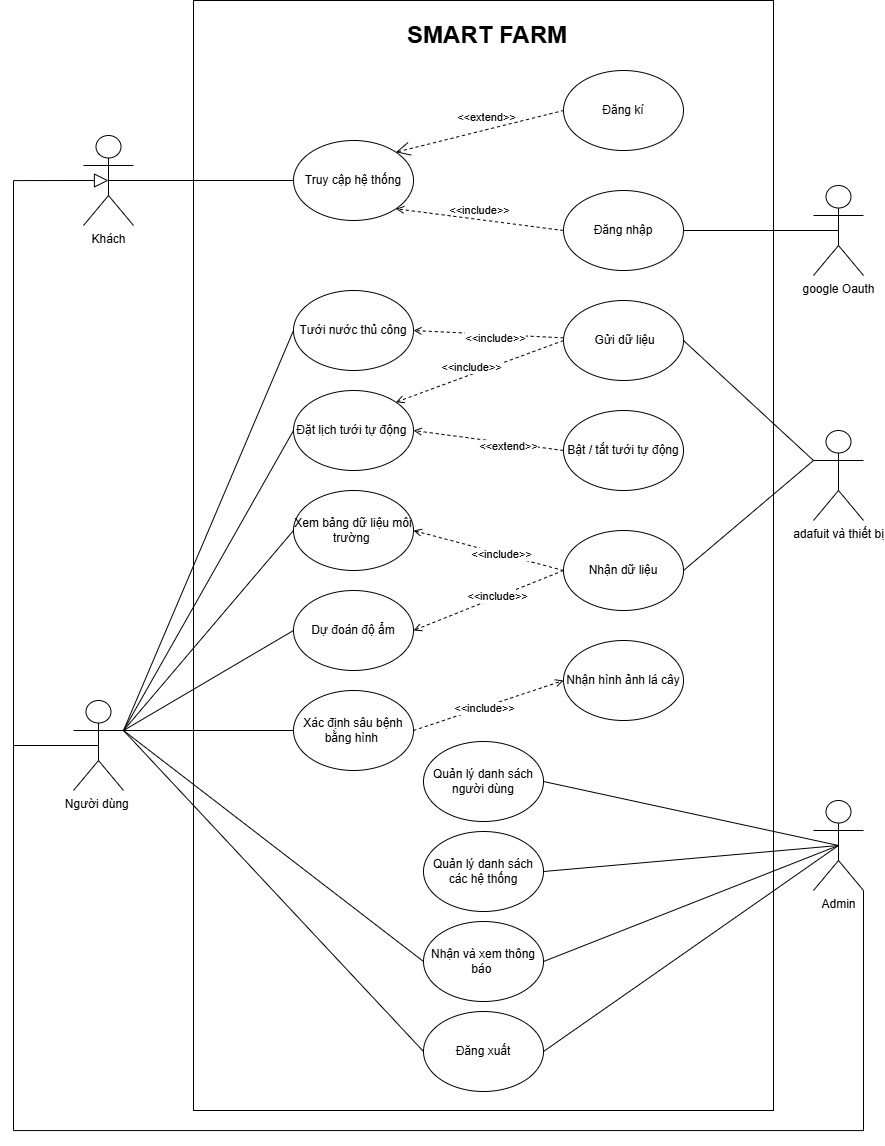
\includegraphics[width=0.8\linewidth]{./Pictures/Task_3/usecase.png}
	\caption{Use-case diagram -- Toàn bộ hệ thống}
\end{figure}
\subsubsection{Details (Scenario)}
%TODO
bsubsub{Truy cập hệ thống}
\setlist[enumerate]{leftmargin=*,topsep=0pt,itemsep=2pt,parsep=0pt}
\setlist[itemize]{leftmargin=*,topsep=0pt,itemsep=2pt,parsep=0pt}
\begin{longtable}{|P{4.8cm}|m{10cm}|}\hline 		
	\texttt{Use-case ID} & UC--01\\
	\hline
	%%%%%%%%%%%%%%%
	\texttt{Use-case Name} & Truy cập hệ thống\\
	\hline
	%%%%%%%%%%%%%%%
	\texttt{Use-case Overview} & Xác thực khách truy cập hệ thống và phân quyền người dùng.
	\\
	\hline
	\texttt{Actors} & Guest (Khách)
	\\
	\hline
	\texttt{Preconditions} & Khách truy cập hệ thống thành công và hệ thống hoạt động bình thường.
	\\
	\hline
	\texttt{Trigger} & Khách chọn nút đăng nhập hoặc đăng kí tài khoản.\\
	\hline
	\texttt{Basic flow} &
	\begin{enumerate}
		\item Khách truy cập hệ thống.
		\item Khách chọn hình thức đăng nhập (trực tiếp hoặc Google account)
		\item Nếu chọn đăng nhập trực tiếp, chọn mục ``Đăng nhập''.
		\item Khách nhập thông tin đăng nhập vào ô tương ứng (tên đăng nhập/ mật khẩu).
		\item Hệ thống đối chiếu thông tin đăng nhập của khách với dữ liệu được lưu ở database.
		\item Nếu khớp thông tin, hệ thống sẽ phân quyền cho khách là người dùng hoặc là admin.
		\item Chuyển người đó tới giao diện tương ứng với vai trò đã phân (user/ admin).
	\end{enumerate}
	\\
	\hline
	\texttt{Post conditions} & 
	Người dùng/ admin truy cập được hệ thống với giao diện tương ứng.
	\\
	\hline
	\texttt{Alterative flow} & 
	\begin{enumerate}[label = A\arabic*.]
		\item Ở bước 3, nếu chọn đăng nhập theo Google account thì hệ thống chuyển hướng người dùng đến trang xác thực của google và Google Oauth sẽ xác thực tài khoản.
		\item Ở bước 3, nếu chọn đăng nhập trực tiếp mà chưa có tài khoản thì khách chọn mục ``đăng kí'' để điền thông tin người dùng, tên đăng nhập và mật khẩu.
	\end{enumerate}
	\\
	\hline
	\texttt{Exception flow} & 
	\begin{enumerate}[label = E\arabic*:]
		\item Ở bước 6, nếu thông tin không khớp thì hệ thống báo lỗi ``tài khoản không đúng tên đăng nhập hoặc mật khẩu'' và khách phải nhập lại thông tin đăng nhập.
		\item Ở bước 7, nếu thông tin đăng nhập không khớp thì vẫn giữ nguyên màn hình đăng nhập.
	\end{enumerate}
	\\
	\hline
	\texttt{Special requirements} & Không có.\\
	\hline
	\texttt{Extension points} & Không có.\\
	\hline
	
	\caption{\label{table2}Đặc tả cho Use-case dự đoán độ ẩm}
\end{longtable}
\subsubsubsection{Dự đoán độ ẩm}
\setlist[enumerate]{leftmargin=*,topsep=0pt,itemsep=2pt,parsep=0pt}
\setlist[itemize]{leftmargin=*,topsep=0pt,itemsep=2pt,parsep=0pt}
\begin{longtable}{|P{4.8cm}|m{10cm}|}\hline 		
	\texttt{Use-case ID} & UC--02\\
	\hline
	%%%%%%%%%%%%%%%
	\texttt{Use-case Name} & Dự đoán độ ẩm\\
	\hline
	%%%%%%%%%%%%%%%
	\texttt{Use-case Overview} & Hệ thống dự đoán độ ẩm đất dựa trên dữ liệu từ cảm biến độ ẩm đất và cảm biến nhiệt độ -- độ ẩm DHT20
	\\
	\hline
	\texttt{Actors} & User
	\\
	\hline
	\texttt{Preconditions} & Hệ thống đã kết nối Internet và cảm biến hoạt động bình thường.
	\\
	\hline
	\texttt{Trigger} & Người dùng chọn chức năng dự đoán độ ẩm trên dashboard\\
	\hline
	\texttt{Basic flow} &
	\begin{enumerate}
		\item Người dùng truy cập dashboard.
		\item Người dùng chọn chức năng ``Dự đoán độ ẩm''.
		\item Hệ thống thu thập dữ liệu từ cảm biến độ ẩm đất.
		\item Hệ thống thu thập dữ liệu nhiệt độ và độ ẩm không khí từ cảm biến DHT20.
		\item Hệ thống gửi dữ liệu đến server xử lý.
		\item Server phân tích dữ liệu và thực hiện dự đoán độ ẩm đất.
		\item Server gửi kết quả dự đoán về hệ thống.
		\item Hệ thống hiển thị kết quả dự đoán trên dashboard.
	\end{enumerate}
	\\
	\hline
	\texttt{Post conditions} & 
	Hệ thống hiển thị kết quả dự đoán độ ẩm
	\\
	\hline
	\texttt{Alterative flow} & Tại bước 1 nếu hệ thống được cấu hình dự đoán tự động theo chu kỳ thì hệ thống tự động thu thập dữ liệu và thực hiện các bước 3 → 8 mà không cần người dùng kích hoạt.\\
	\hline
	\texttt{Exception flow} & 
	\begin{enumerate}[label = E\arabic*:]
		\item Tại bước 3 nếu cảm biến độ ẩm đất không gửi dữ liệu thì hệ thống hiển thị thông báo lỗi và dừng quá trình dự đoán.
		\item Tại bước 5 nếu hệ thống không kết nối được với server thì quá trình xử lý dữ liệu bị hủy và hệ thống hiển thị thông báo lỗi.
	\end{enumerate}
	\\
	\hline
	\texttt{Special requirements} & Không có.\\
	\hline
	\texttt{Extension points} & Không có.\\
	\hline
	
	\caption{\label{table3}Đặc tả cho Use-case dự đoán độ ẩm}
\end{longtable}
\subsubsubsection{Xác định sâu bệnh dựa trên hình ảnh}
%TODO
\setlist[enumerate]{leftmargin=*,topsep=0pt,itemsep=2pt,parsep=0pt}
\setlist[itemize]{leftmargin=*,topsep=0pt,itemsep=2pt,parsep=0pt}
\begin{longtable}{|P{4.8cm}|m{10cm}|}\hline 		
	\texttt{Use-case ID} & UC--03\\
	\hline
	%%%%%%%%%%%%%%%
	\texttt{Use-case Name} & Use-case Xác định sâu bệnh dựa trên hình ảnh\\
	\hline
	%%%%%%%%%%%%%%%
	\texttt{Use-case Overview} & Hệ thống nhận hình ảnh cây trồng từ người dùng hoặc camera và sử dụng mô hình AI để phân tích, xác định loại sâu bệnh có thể xuất hiện trên cây.
	\\
	\hline
	\texttt{Actors} & User
	\\
	\hline
	\texttt{Preconditions} & 
	\begin{enumerate}[label = \arabic*.]
		\item Hệ thống đã kết nối Internet.
		\item Camera hoặc chức năng tải ảnh hoạt động bình thường.
		\item Server AI sẵn sàng xử lý dữ liệu.
	\end{enumerate}
	\\
	\hline
	\texttt{Trigger} & Người dùng chọn chức năng ``Xác định sâu bệnh'' trên dashboard.\\
	\hline
	\texttt{Basic flow} &
	\begin{enumerate}
		\item Người dùng truy cập dashboard.
		\item Người dùng chọn chức năng ``Xác định sâu bệnh''.
		\item Người dùng chụp ảnh cây trồng hoặc tải ảnh từ thiết bị lên hệ thống.
		\item Hệ thống gửi hình ảnh đến server xử lý.
		\item Server phân tích hình ảnh bằng mô hình AI.
		\item Server xác định loại sâu bệnh (nếu có).
		\item Server gửi kết quả dự đoán về hệ thống.
		\item Hệ thống hiển thị kết quả nhận diện sâu bệnh trên dashboard.
	\end{enumerate}
	\\
	\hline
	\texttt{Post conditions} & 
	Hệ thống hiển thị kết quả nhận diện sâu bệnh và thông tin liên quan cho người dùng.
	\\
	\hline
	\texttt{Alterative flow} & Tại bước 3 nếu hệ thống được cấu hình sử dụng camera tự động thì camera sẽ định kỳ chụp ảnh và gửi lên server để phân tích mà không cần người dùng thực hiện.\\
	\hline
	\texttt{Exception flow} & 
	\begin{enumerate}[label = E\arabic*:]
		\item Tại bước 3 nếu người dùng không tải ảnh hoặc camera không hoạt động thì hệ thống hiển thị thông báo lỗi và yêu cầu thử lại.
		\item Tại bước 4 nếu hệ thống không gửi được dữ liệu đến server thì quá trình phân tích bị hủy và hệ thống hiển thị thông báo lỗi.
	\end{enumerate}
	\\
	\hline
	\texttt{Special requirements} & Không có.\\
	\hline
	\texttt{Extension points} & Không có.\\
	\hline
	
	\caption{\label{table4}Đặc tả cho Use-case Xác định sâu bệnh dựa trên hình ảnh}
\end{longtable}
\subsubsubsection{Xem bảng dữ liệu môi trường}
%TODO
\setlist[enumerate]{leftmargin=*,topsep=0pt,itemsep=2pt,parsep=0pt}
\setlist[itemize]{leftmargin=*,topsep=0pt,itemsep=2pt,parsep=0pt}
\begin{longtable}{|P{4.8cm}|m{10cm}|}\hline 		
	\texttt{Use-case ID} & UC--04\\
	\hline
	%%%%%%%%%%%%%%%
	\texttt{Use-case Name} & Xem bảng dữ liệu môi trường\\
	\hline
	%%%%%%%%%%%%%%%
	\texttt{Use-case Overview} & Người dùng xem các thông số môi trường được thu thập từ hệ thống cảm biến như nhiệt độ không khí, độ ẩm không khí và độ ẩm đất.
	\\
	\hline
	\texttt{Actors} & User
	\\
	\hline
	\texttt{Preconditions} & Hệ thống đang thu thập dữ liệu từ cảm biến
	\\
	\hline
	\texttt{Trigger} & Người dùng truy cập dashboard\\
	\hline
	\texttt{Basic flow} &
	\begin{enumerate}
		\item Người dùng truy cập dashboard.
		\item Hệ thống yêu cầu dữ liệu từ các cảm biến.
		\item Hệ thống nhận dữ liệu nhiệt độ và độ ẩm không khí từ cảm biến.
		\item Hệ thống nhận dữ liệu từ cảm biến độ ẩm đất.
		\item Hệ thống xử lý dữ liệu.
		\item Hệ thống hiển thị dữ liệu trên dashboard dưới dạng bảng hoặc biểu đồ.
	\end{enumerate}
	\\
	\hline
	\texttt{Post conditions} & 
	Dữ liệu môi trường được hiển thị cho người dùng
	\\
	\hline
	\texttt{Alterative flow} & Tại bước 6 nếu người dùng chọn xem dữ liệu lịch sử thì hệ thống hiển thị biểu đồ dữ liệu môi trường theo thời gian.\\
	\hline
	\texttt{Exception flow} & 
	\begin{enumerate}[label = E\arabic*:]
		\item Tại bước 3 hoặc bước 4 nếu hệ thống không nhận được dữ liệu từ cảm biến thì dashboard hiển thị trạng thái ``No Data''.
		\item Tại bước 2 nếu dashboard không kết nối được server thì dữ liệu không thể hiển thị và hệ thống thông báo lỗi.
	\end{enumerate}
	\\
	\hline
	\texttt{Special requirements} & Không có.\\
	\hline
	\texttt{Extension points} & Không có.\\
	\hline
	
	\caption{\label{table5}Đặc tả cho Use-case Xem bảng dữ liệu môi trường}
\end{longtable}
\subsubsubsection{Tưới nước thủ công}
%TODO
\setlist[enumerate]{leftmargin=*,topsep=0pt,itemsep=2pt,parsep=0pt}
\setlist[itemize]{leftmargin=*,topsep=0pt,itemsep=2pt,parsep=0pt}
\begin{longtable}{|P{4.8cm}|m{10cm}|}\hline 		
	\texttt{Use-case ID} & UC--05\\
	\hline
	%%%%%%%%%%%%%%%
	\texttt{Use-case Name} & Use-case Tưới nước thủ công\\
	\hline
	%%%%%%%%%%%%%%%
	\texttt{Use-case Overview} & Người dùng có thể chủ động bật hoặc tắt hệ thống tưới nước thông qua dashboard để tưới cây ngay lập tức.
	\\
	\hline
	\texttt{Actors} & User
	\\
	\hline
	\texttt{Preconditions} & 
	\begin{enumerate}[label = \arabic*.]
		\item Hệ thống đang hoạt động bình thường.
		\item Người dùng đã truy cập dashboard.
		\item Máy bơm nước được kết nối với hệ thống.
	\end{enumerate}
	\\
	\hline
	\texttt{Trigger} & Người dùng chọn chức năng ``Tưới nước thủ công'' trên dashboard.\\
	\hline
	\texttt{Basic flow} &
	\begin{enumerate}
		\item Người dùng truy cập dashboard.
		\item Người dùng chọn chức năng ``Tưới nước thủ công''.
		\item Hệ thống hiển thị nút điều khiển bật/tắt máy bơm.
		\item Người dùng chọn bật máy bơm.
		\item Hệ thống gửi tín hiệu điều khiển đến bộ điều khiển máy bơm.
		\item Máy bơm bắt đầu hoạt động và tưới cây.
		\item Khi người dùng chọn tắt máy bơm, hệ thống gửi tín hiệu dừng.
		\item Máy bơm ngừng hoạt động.
	\end{enumerate}
	\\
	\hline
	\texttt{Post conditions} & 
	Máy bơm nước được kích hoạt hoặc tắt theo thao tác của người dùng.
	\\
	\hline
	\texttt{Alterative flow} & Tại bước 4 nếu người dùng đặt thời gian tưới cụ thể thì hệ thống tự động tắt máy bơm sau khi hết thời gian đã chọn.\\
	\hline
	\texttt{Exception flow} & 
	\begin{enumerate}[label = E\arabic*:]
		\item Tại bước 5 nếu hệ thống không gửi được tín hiệu điều khiển đến máy bơm thì hệ thống hiển thị thông báo lỗi.
		\item Tại bước 6 nếu máy bơm không phản hồi thì hệ thống hiển thị trạng thái lỗi và yêu cầu người dùng kiểm tra thiết bị.
	\end{enumerate}
	\\
	\hline
	\texttt{Special requirements} & Không có.\\
	\hline
	\texttt{Extension points} & Không có.\\
	\hline
	
	\caption{\label{table6}Đặc tả cho Use-case Tưới nước thủ công}
\end{longtable}

\subsubsubsection{Đặt lịch tưới nước tự động}
%TODO
\setlist[enumerate]{leftmargin=*,topsep=0pt,itemsep=2pt,parsep=0pt}
\setlist[itemize]{leftmargin=*,topsep=0pt,itemsep=2pt,parsep=0pt}
\begin{longtable}{|P{4.8cm}|m{10cm}|}\hline 		
	\texttt{Use-case ID} & UC--06\\
	\hline
	%%%%%%%%%%%%%%%
	\texttt{Use-case Name} & Đặt lịch tưới nước tự động\\
	\hline
	%%%%%%%%%%%%%%%
	\texttt{Use-case Overview} & Người dùng thiết lập lịch tưới nước tự động cho hệ thống. Khi đến thời gian đã đặt, hệ thống sẽ kích hoạt máy bơm để tưới cây.
	\\
	\hline
	\texttt{Actors} & User
	\\
	\hline
	\texttt{Preconditions} & Hệ thống đã kết nối Internet và máy bơm nước hoạt động bình thường.
	\\
	\hline
	\texttt{Trigger} & Người dùng chọn chức năng đặt lịch tưới nước\\
	\hline
	\texttt{Basic flow} &
	\begin{enumerate}
		\item Người dùng truy cập dashboard.
		\item Người dùng chọn chức năng ``Đặt lịch tưới nước''.
		\item Người dùng nhập thời gian bắt đầu và thời gian tưới.
		\item Hệ thống lưu lịch tưới.
		\item Khi đến thời gian đã đặt, hệ thống kích hoạt máy bơm nước.
		\item Sau khi hết thời gian tưới, hệ thống tắt máy bơm.
	\end{enumerate}
	\\
	\hline
	\texttt{Post conditions} & 
	Lịch tưới được lưu và hệ thống thực hiện tưới tự động
	\\
	\hline
	\texttt{Alterative flow} & 
	\begin{enumerate}[label = A\arabic*:]
		\item Tại bước 4 nếu người dùng muốn thay đổi lịch tưới thì hệ thống cho phép chỉnh sửa và lưu lại lịch mới.
		\item Tại bước 2 nếu người dùng tắt chế độ tưới tự động thì hệ thống không thực hiện lịch tưới đã đặt.
	\end{enumerate}
	\\
	\hline
	\texttt{Exception flow} & 
	\begin{enumerate}[label = E\arabic*:]
		\item Tại bước 3 nếu thời gian người dùng nhập không hợp lệ thì hệ thống yêu cầu người dùng nhập lại.
		\item Tại bước 5 nếu máy bơm không phản hồi thì hệ thống hiển thị thông báo lỗi và không thực hiện tưới nước.
	\end{enumerate}
	\\
	\hline
	\texttt{Special requirements} & Không có.\\
	\hline
	\texttt{Extension points} & Không có.\\
	\hline
	
	\caption{\label{table7}Đặc tả cho Use-case Đặt lịch tưới nước tự động}
\end{longtable}
\subsubsubsection{Nhận và xem thông báo}
%TODO
\setlist[enumerate]{leftmargin=*,topsep=0pt,itemsep=2pt,parsep=0pt}
\setlist[itemize]{leftmargin=*,topsep=0pt,itemsep=2pt,parsep=0pt}
\begin{longtable}{|P{4.8cm}|m{10cm}|}\hline 		
	\texttt{Use-case ID} & UC--07\\
	\hline
	%%%%%%%%%%%%%%%
	\texttt{Use-case Name} & Use-case Nhận và xem thông báo\\
	\hline
	%%%%%%%%%%%%%%%
	\texttt{Use-case Overview} & Hệ thống gửi thông báo đến người dùng khi xảy ra các sự kiện quan trọng như độ ẩm đất thấp, phát hiện sâu bệnh, lỗi cảm biến hoặc hệ thống tưới nước. Hoặc gửi thông báo đến admin về những thay đổi mà admin đã thực hiện.
	\\
	\hline
	\texttt{Actors} & User, Admin
	\\
	\hline
	\texttt{Preconditions} & 
	\begin{enumerate}[label = \arabic*.]
		\item Hệ thống đã kết nối Internet.
		\item Người dùng/ admin đã đăng nhập vào hệ thống.
	\end{enumerate}
	\\
	\hline
	\texttt{Trigger} & Hệ thống phát hiện một sự kiện cần thông báo.\\
	\hline
	\texttt{Basic flow} &
	\begin{enumerate}
		\item Hệ thống phát hiện sự kiện cần thông báo.
		\item Hệ thống tạo thông báo với nội dung tương ứng.
		\item Hệ thống gửi thông báo đến dashboard hoặc ứng dụng của người dùng hoặc admin.
		\item Người dùng hoặc admin mở mục thông báo trên dashboard.
		\item Hệ thống hiển thị danh sách các thông báo.
		\item Người dùng hoặc admin chọn một thông báo để xem chi tiết.
	\end{enumerate}
	\\
	\hline
	\texttt{Post conditions} & 
	Người dùng hoặc admin nhận được và xem nội dung thông báo.
	\\
	\hline
	\texttt{Alterative flow} & Tại bước 3 nếu người dùng bật thông báo qua email hoặc ứng dụng di động thì hệ thống gửi thông báo qua các kênh này.\\
	\hline
	\texttt{Exception flow} & 
	\begin{enumerate}[label = E\arabic*:]
		\item Tại bước 3 nếu hệ thống không kết nối được Internet thì thông báo sẽ được lưu lại và gửi khi kết nối được khôi phục.
		\item Tại bước 4 nếu người dùng chưa đăng nhập thì hệ thống yêu cầu đăng nhập trước khi xem thông báo.
	\end{enumerate}
	\\
	\hline
	\texttt{Special requirements} & Không có.\\
	\hline
	\texttt{Extension points} & Không có.\\
	\hline
	
	\caption{\label{table8}Đặc tả cho Use-case Nhận và xem thông báo}
\end{longtable}

\subsubsubsection{Đăng xuất}
%TODO
\setlist[enumerate]{leftmargin=*,topsep=0pt,itemsep=2pt,parsep=0pt}
\setlist[itemize]{leftmargin=*,topsep=0pt,itemsep=2pt,parsep=0pt}
\begin{longtable}{|P{4.8cm}|m{10cm}|}\hline 		
	\texttt{Use-case ID} & UC--08\\
	\hline
	%%%%%%%%%%%%%%%
	\texttt{Use-case Name} & Use-case Đăng xuất\\
	\hline
	%%%%%%%%%%%%%%%
	\texttt{Use-case Overview} & Người dùng/ admin chọn đăng xuất, hệ thống hiển thị lại màn hình đăng nhập và xóa bỏ phân quyền người dùng hiện tại.
	\\
	\hline
	\texttt{Actors} & User, admin
	\\
	\hline
	\texttt{Preconditions} & 
	\begin{enumerate}[label = \arabic*.]
		\item Người dùng đã đăng nhập vào hệ thống.
		\item Người dùng, admin đang ở trong hệ thống.
	\end{enumerate}
	\\
	\hline
	\texttt{Trigger} & Người dùng/ admin nhấn vào nút ``đăng xuất''.\\
	\hline
	\texttt{Basic flow} &
	\begin{enumerate}
		\item Người dùng/ admin nhấn vào nút đăng xuất.
		\item Hệ thống hiển thị thông báo yêu cầu xác nhận việc đăng xuất.
		\item Nếu chấp nhận, hệ thống xóa bỏ phân quyền hiện tại và chuyển hướng về giao diện đăng nhập.
	\end{enumerate}
	\\
	\hline
	\texttt{Post conditions} & 
	Người dùng/ admin bị xóa bỏ phân quyền và trở lại là khách; hệ thống chuyển hướng về màn hình đăng nhập.
	\\
	\hline
	\texttt{Alterative flow} & Tại bước 3, nếu không chấp nhận thì hệ thống hủy bỏ việc đăng xuất và vẫn giữ nguyên quyền của người dùng này.\\
	\hline
	\texttt{Exception flow} & 
	Không có
	\\
	\hline
	\texttt{Special requirements} & Không có.\\
	\hline
	\texttt{Extension points} & Không có.\\
	\hline
	
	\caption{\label{table9}Đặc tả cho Use-case Đăng xuất}
\end{longtable}
\subsection{Use-case chi tiết cho role Admin}
\subsubsection{Diagram}
%TODO
\begin{figure}[H]
	\centering
	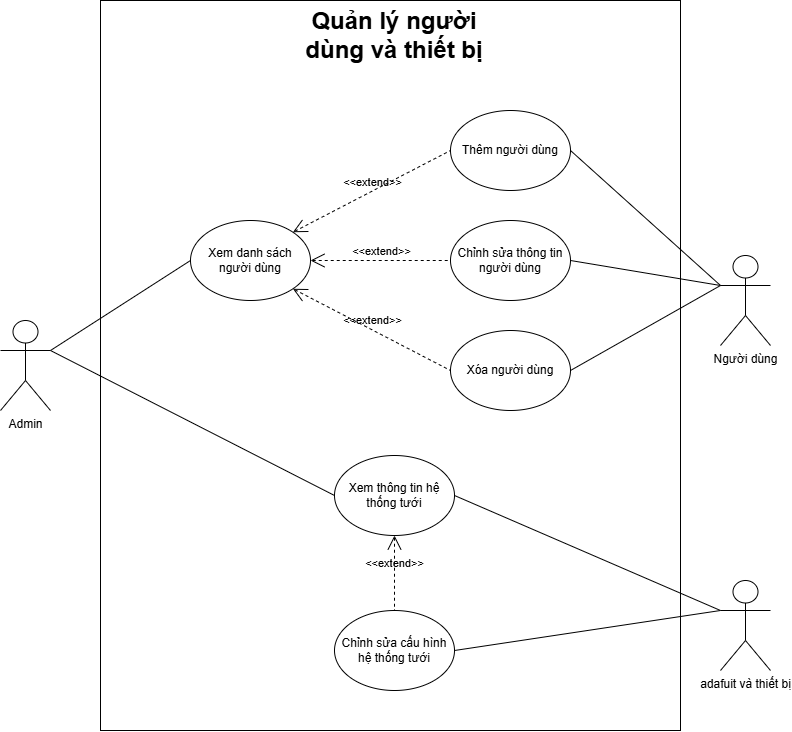
\includegraphics[width=0.8\linewidth]{./Pictures/Task_3/usecase_admin.png}
	\caption{Use-case diagram -- chi tiết cho role Admin}
\end{figure}

\subsubsection{Details (Scenario)}
%TODO
\subsubsubsection{Xem danh sách người dùng}
\setlist[enumerate]{leftmargin=*,topsep=0pt,itemsep=2pt,parsep=0pt}
\setlist[itemize]{leftmargin=*,topsep=0pt,itemsep=2pt,parsep=0pt}
\begin{longtable}{|P{4.8cm}|m{10cm}|}\hline 		
	\texttt{Use-case ID} & UC--B01\\
	\hline
	%%%%%%%%%%%%%%%
	\texttt{Use-case Name} & Xem danh sách người dùng\\
	\hline
	%%%%%%%%%%%%%%%
	\texttt{Use-case Overview} & Admin có thể xem danh sách các người dùng đã đăng kí tài khoản vào hệ thống, ngoài ra còn có thể thêm người dùng, chỉnh sửa thông tin hoặc xóa tài khoản người dùng đã đăng kí trước đó.
	\\
	\hline
	\texttt{Actors} & Admin, users
	\\
	\hline
	\texttt{Preconditions} & Admin đăng nhập thành công vào hệ thống.
	\\
	\hline
	\texttt{Trigger} & Admin truy cập vào mục quản lý người dùng.\\
	\hline
	\texttt{Basic flow} &
	\begin{enumerate}
		\item Admin truy cập vào mục quản lý người dùng.
		\item Admin chọn các chức năng đặc quyền: thêm, chỉnh sửa thông tin, xóa người dùng.
		\item Nếu chọn thêm người dùng, admin có thể tạo một tài khoản người dùng mới bằng việc thêm tên đăng nhập, mật khẩu tương ứng. Hệ thống ghi nhận và thêm vào cơ sở dữ liệu.
	\end{enumerate}
	\\
	\hline
	\texttt{Post conditions} & 
	Hệ thống cập nhật lại thông tin tương ứng mà admin đã thao tác.
	\\
	\hline
	\texttt{Alterative flow} & 
	\begin{enumerate}[label = A\arabic*.]
		\item Ở bước 3, nếu admin chọn chỉnh sửa thông tin người dùng thì admin có thể chỉnh sửa thông tin cá nhân, tên đăng nhập và mật khẩu người dùng.
		\item Ở bước 3, nếu admin chọn xoá người dùng thì hệ thống sẽ xóa toàn bộ thông tin của người dùng trong cơ sở dữ liệu.
	\end{enumerate}
	\\
	\hline
	\texttt{Exception flow} & 
	\begin{enumerate}[label = E\arabic*:]
		\item Ở bước 2, nếu admin tìm thông tin của người dùng không tồn tại trong cơ sở dữ liệu hiện tại thì hệ thống báo lỗi.
	\end{enumerate}
	\\
	\hline
	\texttt{Special requirements} & Không có.\\
	\hline
	\texttt{Extension points} & Không có.\\
	\hline
	
	\caption{\label{table10}Đặc tả cho Use-case Xem danh sách người dùng}
\end{longtable}

\subsubsubsection{Xem danh sách người dùng}
\setlist[enumerate]{leftmargin=*,topsep=0pt,itemsep=2pt,parsep=0pt}
\setlist[itemize]{leftmargin=*,topsep=0pt,itemsep=2pt,parsep=0pt}
\begin{longtable}{|P{4.8cm}|m{10cm}|}\hline 		
	\texttt{Use-case ID} & UC--B02\\
	\hline
	%%%%%%%%%%%%%%%
	\texttt{Use-case Name} & Xem thông tin hệ thống tưới\\
	\hline
	%%%%%%%%%%%%%%%
	\texttt{Use-case Overview} & Admin có thể xem và chỉnh sửa các thông số của các thiết bị cũng như cách bố trí các thành phần trong hệ thống.
	\\
	\hline
	\texttt{Actors} & Admin, adafruit và thiết bị
	\\
	\hline
	\texttt{Preconditions} & Admin đăng nhập thành công vào hệ thống.
	\\
	\hline
	\texttt{Trigger} & Admin truy cập vào mục ``quản lý thiết bị và hệ thống''.\\
	\hline
	\texttt{Basic flow} &
	\begin{enumerate}
		\item Admin truy cập vào mục ``quản lý thiết bị và hệ thống''.
		\item Admin chọn mục xem thông tin hệ thống tưới.
		\item Hệ thống truy xuất dữ liệu cấu hình thiết bị từ Adafruit và cơ sở dữ liệu.
		\item Hệ thống hiển thị danh sách các thiết bị trong hệ thống tưới (cảm biến độ ẩm đất, cảm biến DHT20, máy bơm nước) cùng với trạng thái hoạt động và các thông số cấu hình hiện tại.
		\item Admin xem chi tiết thông tin của từng thiết bị bao gồm: tên thiết bị, trạng thái kết nối, giá trị đọc được, ngưỡng hoạt động và lịch sử hoạt động.
	\end{enumerate}
	\\
	\hline
	\texttt{Post conditions} & 
	Hệ thống cập nhật lại thông tin tương ứng mà admin đã thao tác.
	\\
	\hline
	\texttt{Alterative flow} & 
	\begin{enumerate}[label = A\arabic*.]
		\item Ở bước 5, nếu admin chọn chỉnh sửa cấu hình hệ thống tưới thì hệ thống cho phép admin thay đổi các thông số như: ngưỡng độ ẩm kích hoạt tưới, thời gian tưới, tần suất đọc cảm biến. Sau khi chỉnh sửa, hệ thống gửi cấu hình mới đến Adafruit để cập nhật cho thiết bị.
	\end{enumerate}
	\\
	\hline
	\texttt{Exception flow} & 
	\begin{enumerate}[label = E\arabic*:]
		\item Ở bước 3, nếu hệ thống không kết nối được tới Adafruit thì báo lỗi.
	\end{enumerate}
	\\
	\hline
	\texttt{Special requirements} & Không có.\\
	\hline
	\texttt{Extension points} & Không có.\\
	\hline
	
	\caption{\label{table11}Đặc tả cho Use-case Xem thông tin hệ thống tưới}
\end{longtable}